\section{The Idea of Stream Ciphers}

Stream ciphers are one of two major symmetric encryption methods. They serve a different purpose than block ciphers, the second symmetric encryption method. The primary intent is to encrypt and decrypt messages approximately synchronously between the sender and receiver of a message. To achieve this, the message is not first divided into blocks and pre-processed before it is ciphered, as is the case with block ciphers. Instead, stream ciphers encrypt or decrypt the plaintext or ciphertext directly. \cite[p. 223]{Schneier.2006} \\

A prerequisite for this is a theoretically infinite, ideally truly random binary sequence. To encrypt the data, the sender combines the plaintext bitwise exclusive-or (XOR) with the random sequence. The recipient decrypts the ciphertext by also combining it bitwise exclusive-or with the same random sequence used by the sender.
\begin{figure}[h]
	\centering
	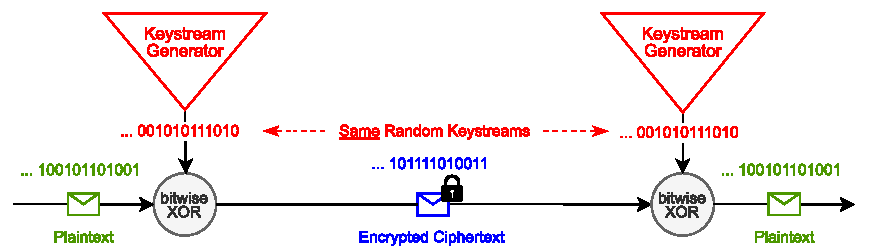
\includegraphics[width=1\textwidth]{carl/figures/figure_1_new_svg-raw.pdf}
	\caption{Stream cipher as a symmetric encryption method, based on \cite[p. 232]{Schneier.2006}}
	\label{fig:Figure_1}
\end{figure}
\\ This only works if both communication partners have the same random sequence. This is a characteristic of symmetric encryption. \cite[pp. 319-320]{Schmeh.2016} This problem could be trivially solved by the sender first generating a true random sequence of sufficient length and transmitting it to the recipient. However since this key sequence can also be seen as plaintext which must be transmitted securely, the situation results in a stream cipher with exactly the same problem as before.
\subsection{"True Pseudorandomness"}
The central question that arises is: How can truly random numbers be generated by means of a computer, based on a short key? \cite[p. 53]{Beutelspacher.2005} Without starting a philosophical discussion, it is necessary to define what characterizes a truly random bit sequence. \\

This can be described using an analogy to a Laplacean experiment, like the sequences of fair coin tosses: Within this sequence, the values $0$ and $1$ each occur with probability $0.5$. In addition, there is no way to derive information about the rest of the sequence from knowledge of an arbitrarily long initial piece of the sequence. To predict the next bit, an attacker must thus have no better chance of success than $0.5$. To achieve equal distribution of the bits, the experiment must be conducted theoretically for a long time. Combining a given message $M$ with this truly random sequence XOR results in a truly random ciphertext $C$. Based on this information, a so-called \textit{perfect cipher system} is characterized by the fact that the a priori probability $P\left(M\right)$ is equal to the a posteriori probability $P({M}\mid{C})$ resulting in $P({M}\mid{C})\ = P({M})$. \cite[pp. 52-23]{Ertel.2020}

\pagebreak

The real question is in fact: Can a computer generate numbers that only look truly random? Due to the determinism of a PC, which can be represented as a finite state machine, truly random numbers can never be generated. It is only possible to generate deterministic, so-called \textit{pseudorandom numbers} (PRN). After the input of one or more initialization numbers, a \textit{pseudorandom number generator} (PRNG) generates this pseudorandom number sequence. A deterministic inner state is used for this purpose. \cite[pp. 195-196]{Ertel.2020} In the following chapters it will be shown that a stream cipher can be interpreted as a PRNG according to these criteria. As can be seen in Figure \ref{fig:Figure_2}, a stream cipher has this inner state of the PRNG. Initially, it is filled with a short key that could be exchanged using an asymmetric cryptosystem. A stream cipher uses the key to generate and output the pseudorandom \textit{keystream} or \textit{running-key} bitwise or bytewise. \cite[p. 233]{Schneier.2006} \\

\begin{figure}[h]
	\centering
	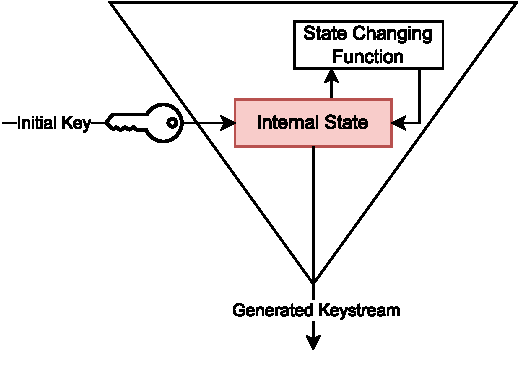
\includegraphics[width=0.48\textwidth]{carl/figures/figure_2_new_svg-raw.pdf}
	\caption{A stream cipher generates the keystream with the help of the initial key, using an inner state. Based on \cite[p. 234]{Schneier.2006}}
	\label{fig:Figure_2}
\end{figure}

Optimally, this generated bit sequence should have the same statistical properties as truly random bits. To estimate this statistical quality, a series of statistical tests exist. Pioneering for the evaluation of pseudorandom numbers were the \textit{Golomb-postulates} formulated in the 1960s by the American mathematician Solomon W. Golomb. \cite[p. 43]{Golomb.1967} In order to keep the scope of this paper concise, the focus is not on this topic.\\

Ultimately, it should not be computationally feasible for an attacker to determine the prospective  sequence. No matter how many bits of the keystream one has, the probability of guessing the next bit correctly should not be better than half.
